%%%%%%%%%%%%%%%%%%%%%%%%
%%                    %%
%%  PROJECT-SPECIFIC  %%
%%                    %%
%%%%%%%%%%%%%%%%%%%%%%%%

% Fix typo to enable italics in captions.
% https://tex.stackexchange.com/questions/453542/unable-to-use-texit-in-caption
\renewcommand{\sfdefault}{phv}

%%%%%%%%%%%%
% PACKAGES %
%%%%%%%%%%%%
%https://tex.stackexchange.com/questions/5293/how-to-patch-a-package
%\let\href\undefined
%\usepackage{layout}
%\usepackage[capitalize]{cleveref}
\usepackage{xspace}
\usepackage{amsmath}
\usepackage{amssymb}
\usepackage{amsthm}

\usepackage{latexsym}  % \leadsto
%\usepackage{subcaption}  % for subfigure
%\usepackage[caption=false]{subfig}  % deprecated

\usepackage{booktabs}   % tables: toprule, midrule
\usepackage{colortbl}
\usepackage{dsfont} % beautiful 1
\usepackage{float}
\usepackage{ragged2e}
%\usepackage{natbib}

%\usepackage{biblatex}  % \pno for page number \ppno for pageS

\usepackage[]{todonotes}  % [disable]
\usepackage{mathtools}   % smashoperator 

\usepackage{graphicx}
\usepackage{epigraph}
%\usepackage{siunitx}  % aligning to decimal point

\usepackage{svg}
\usepackage{tikz}
\usetikzlibrary{tikzmark,decorations.pathreplacing,calc}
%\usepackage{tabu}% http://ctan.org/pkg/tabu
%\usepackage{xcolor}% http://ctan.org/pkg/xcolor
%\usepackage{tabularx}% http://ctan.org/pkg/tabularx

\usepackage{multirow}   % tables

\usepackage{numprint}   % tables
\npdecimalsign{.}

%\captionsetup{compatibility=false}   % gitlab compilation happy
%\DeclareCaptionLabelSeparator{emdash}{\textemdash}  % solves a caption error

\setcounter{tocdepth}{3}

\usepackage{thmtools}
\usepackage{thm-restate}
\usepackage{etoolbox}
\declaretheorem[name=Theorem]{thm}
\declaretheorem[name=Proposition]{prop}
\declaretheorem[name=Lemma]{lem}
\declaretheorem[name=Definition]{definition}
\declaretheorem[name=Observation]{observation}
\declaretheorem[name=Corollary]{cor}
\declaretheorem[name=Remark]{remark}
% used packages

%%%%%%%%%%%%
%   MATH   %
%%%%%%%%%%%%
% math symbols and operations

%%%%%%%%%%%%%%%
% TEXT FORMAT %
%%%%%%%%%%%%%%%
% commands for text formatting

%%%%%%%%%%%%
%  OTHERS  %
%%%%%%%%%%%%

\newcommand{\A}[0]{A$^\star$\xspace}
\newcommand{\csh}[0]{chaining seed heuristic\xspace}
\newcommand{\Csh}[0]{Chaining seed heuristic\xspace}
\newcommand{\CSH}[0]{CSH\xspace}
\newcommand{\sh}[0]{seed heuristic\xspace}
\newcommand{\Sh}[0]{Seed heuristic\xspace}
\newcommand{\SH}[0]{SH\xspace}
%\newcommand{\mpp}[0]{multiple-path pruning\xspace}
%\newcommand{\Mpp}[0]{Multiple-path pruning\xspace}

\newcommand{\lcs}[0]{\mbox{LCS}\xspace}
\newcommand{\lcskpp}[0]{\mbox{LCSk++}\xspace}
\newcommand{\pa}[0]{pairwise alignment\xspace}
\newcommand{\ed}[0]{\mbox{ed}\xspace}

% tool names
\newcommand{\difftool}[0]{\mbox{\textsc{diff}}\xspace}
\newcommand{\edlib}[0]{\mbox{\textsc{Edlib}}\xspace}
\newcommand{\oldwfa}[0]{\mbox{\textsc{WFA}}\xspace}
\newcommand{\wfa}[0]{\mbox{\textsc{BiWFA}}\xspace}
\newcommand{\seqan}[0]{\mbox{\textsc{SeqAn}}\xspace}
\newcommand{\parasail}[0]{\mbox{\textsc{Parasail}}\xspace}
\newcommand{\astarpa}[0]{\mbox{\textsc{A*PA}}\xspace}
\newcommand{\astarix}[0]{\mbox{\textsc{AStarix}}\xspace}
\newcommand{\dijkstra}[0]{\mbox{Dijkstra}\xspace}


\patchcmd{\paragraph}{\itshape}{\bfseries\boldmath}{}{}

\setlength{\abovecaptionskip}{5pt plus 0pt minus 0pt}

% general math
\newcommand{\Oh}[0]{O}

\newcommand{\seeds}{\mathcal S}
\newcommand{\matches}{\mathcal M}

% Commands for A* functions
\newcommand{\st}[2]{\langle #1, #2 \rangle}
\newcommand{\g}{g^*\!}
\newcommand{\h}{h^*\!}
\newcommand{\ssh}{_{\mathrm{sh}}}
\newcommand{\scsh}{_{\mathrm{csh}}}
\newcommand{\hsh}{h\ssh\!}
\newcommand{\hcsh}{h\scsh\!}
\newcommand{\hshM}{h\ssh^\matches\!}
\newcommand{\hcshM}{h\scsh^\matches\!}
\newcommand{\hh}{\hat h}
\newcommand{\hshS}{\hat h\ssh\!}
\newcommand{\hcshS}{\hat h\scsh\!}
\newcommand{\Path}{\pi^*}

\newcommand{\Pot}{P}
\newcommand{\spot}{r}
\newcommand{\cost}{\operatorname{cost}}
\newcommand{\matchscore}{\operatorname{score}}
\newcommand{\seedscore}{\operatorname{score}}
\newcommand{\statescore}{S}
\newcommand{\chainscore}{S_{\mathrm{chain}}}
\newcommand{\shscore}{S_{\mathrm{sh}}}
\newcommand{\cshscore}{S_{\mathrm{csh}}}

\newcommand{\layer}{\mathcal L}

\newcommand{\start}{\operatorname{start}}

\newcommand{\substr}[3]{#1_{#2{\dots}#3}}

\renewcommand{\path}[2]{(#1{\leadsto}#2)}

% Fig.2
\newcommand{\bluecircle}{
\includegraphics[height=4pt]{imgs/fig2-symbols/blue-circle.pdf}}
\newcommand{\greencircle}{
\includegraphics[height=4pt]{imgs/fig2-symbols/green-circle.pdf}}
\newcommand{\cross}{
\includegraphics[height=4pt]{imgs/fig2-symbols/cross.pdf}}
\newcommand{\seed}{
\includegraphics[width=6pt]{imgs/fig2-symbols/seed.pdf}}
\newcommand{\match}{
\includegraphics[height=4pt]{imgs/fig2-symbols/match.pdf}}
\newcommand{\redcolumn}{
\includegraphics[height=5pt]{imgs/fig2-symbols/red-column.pdf}}
\newcommand{\greencolumn}{
\includegraphics[height=5pt]{imgs/fig2-symbols/green-column.pdf}}

% Fig.3
\newcommand{\bluesquare}{
\includegraphics[height=4pt]{imgs/fig3-symbols/bluesquare.pdf}}
\newcommand{\greensquare}{
\includegraphics[height=4pt]{imgs/fig3-symbols/greensquare.pdf}}
\newcommand{\blackmatch}{
\includegraphics[height=5pt]{imgs/fig3-symbols/blackmatch.pdf}}
\newcommand{\redmatch}{
\includegraphics[height=5pt]{imgs/fig3-symbols/redmatch.pdf}}

% Plots
\newcommand{\edlibsymbol}{
\includegraphics[height=4pt]{imgs/plots-symbols/edlib.pdf}}
\newcommand{\wfasymbol}{
\includegraphics[height=4pt]{imgs/plots-symbols/wfa.pdf}}
\newcommand{\shsymbol}{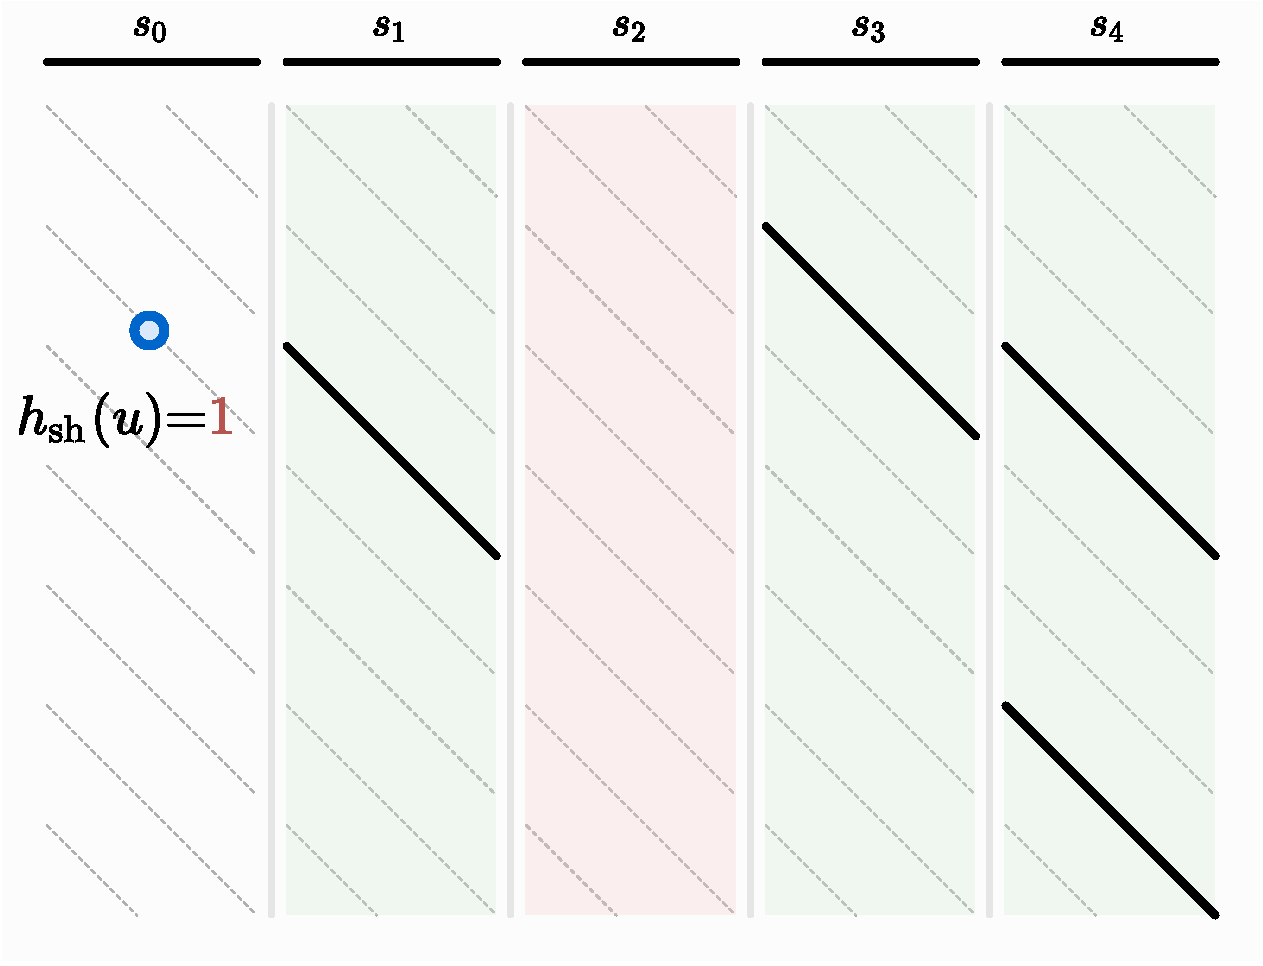
\includegraphics[height=4pt]{imgs/plots-symbols/sh.pdf}}
\newcommand{\shsymbolsq}{
\includegraphics[height=4pt]{imgs/plots-symbols/sh-down.pdf}}
\newcommand{\cshsymbol}{
\includegraphics[height=4pt]{imgs/plots-symbols/csh.pdf}}
\newcommand{\cshsymbolsq}{
\includegraphics[height=4pt]{imgs/plots-symbols/csh-down.pdf}}

% TODO
%\newcommand{\bp}{\unit{\,bp}}
%\newcommand{\kbp}{\unit{\,kbp}}
\newcommand{\bp}{\,bp}
\newcommand{\kbp}{\,kbp}
% TODO: remove \qty and \unit in favor of siunitx
\newcommand{\qty}[2]{#1\ #2}
\newcommand{\unit}[1]{#1} 

% datasets
\newcommand{\datasetOne}{CHM13}
\newcommand{\datasetTwo}{NA12878}

%\newenvironment{proof}{\paragraph{Proof:}}{\hfill$\square$}
